%----------------------------------------------------------------------------------------
%	PACKAGES AND THEMES
%----------------------------------------------------------------------------------------

\documentclass[aspectratio=169]{beamer}

\mode<presentation> {
\usetheme{Madrid}
\usecolortheme{seahorse}

\AtBeginSection[]{
  \begin{frame}
  \vfill
  \centering
  \begin{beamercolorbox}[sep=8pt,center,shadow=true,rounded=true]{title}
    \usebeamerfont{title}\insertsectionhead\par%
  \end{beamercolorbox}
  \vfill
  \end{frame}
}

% To remove the footer line in all slides uncomment next line
%\setbeamertemplate{footline}
% To replace the footer line in all slides with a simple slide count uncomment next line
%\setbeamertemplate{footline}[page number]
% To remove the navigation symbols from the bottom of all slides uncomment next line
\setbeamertemplate{navigation symbols}{}
}

\usepackage{graphicx} % Allows including images
\usepackage{booktabs} % Allows the use of \toprule, \midrule and \bottomrule in tables
\usepackage{caption}
\usepackage{multirow}
\usepackage{adjustbox}

\usepackage[backend=biber, style=authoryear, sorting=nty]{biblatex}
\bibliography{references.bib}
\renewcommand*{\bibfont}{\footnotesize}

\let\oldparencites\parencites
\renewcommand{\parencites}[1]{{\color{gray}\scriptsize \oldparencites{#1}}}

\let\oldcites\cites
\renewcommand{\cites}[1]{{\color{gray}\scriptsize (see \oldcites{#1})}}

\newcommand{\source}[1]{\caption*{\tiny Source: \url{#1}}}

\let\olditemize\itemize
\def\itemize{
    \olditemize
    \itemsep1em
}

\let\oldenumerate\enumerate
\def\enumerate{
    \oldenumerate
    \itemsep1em
}



%----------------------------------------------------------------------------------------
%	TITLE PAGE
%----------------------------------------------------------------------------------------


% The short title appears at the bottom of every slide, the full title is only on the title page
% \title[short title]{long title}
\title{Topic Analysis of Textbooks Using AI}

\author{Coby Simmons}
\institute[Utrecht University]{
Utrecht University
\\ \medskip
\textit{cobysimmons01@gmail.com}
}
\date{31 January 2024}

\graphicspath {{images/}}



\begin{document}

\begin{frame}
\titlepage % Print the title page as the first slide
\end{frame}

%----------------------------------------------------------------------------------------
%	PRESENTATION SLIDES
%----------------------------------------------------------------------------------------


\begin{frame} \frametitle{Aim and Motivation}

\begin{itemize}
    \item focus on the application of AI in identifying and categorising topics in textbooks \pause
    \item construct a domain-dependent, fine-grained topic model \pause
    \item enable enhanced learning experiences via learning object classification, automatic index creation, content personalisation, etc.
\end{itemize}

\end{frame}


\begin{frame} \frametitle{Overview}
\tableofcontents
\end{frame}


\section{Previous Research}

\begin{frame} \frametitle{Modelling of textbooks}

\begin{itemize}
    \item proposal for an intelligent online learning experience: ``Intextbooks'' \\ \parencites{alpizarchacon2020intextbooks}
    \item extraction of knowledge models from PDF textbooks; encoding as TEI\footnote{\url{https://tei-c.org/}} files \\ \parencites{alpizarchacon2020, alpizarchacon2021}
    \item semantic linking and enrichment of glossary \& index \\ \parencites{alpizarchacon2019, alpizarchacon2022}
\end{itemize}

\end{frame}

\begin{frame} \frametitle{Modelling Topics}

\begin{figure}[h]
    \centering
    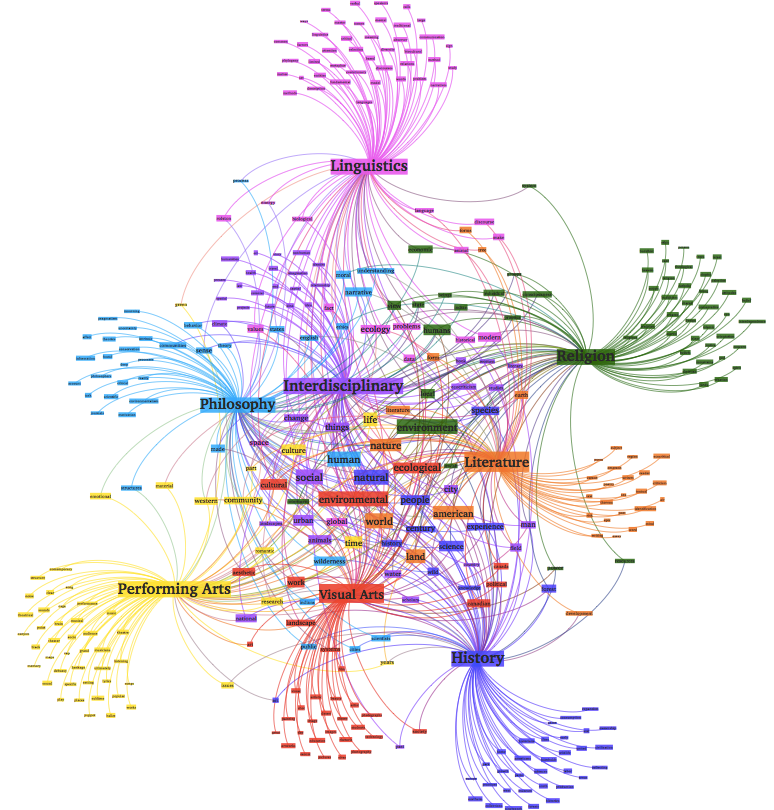
\includegraphics[width=0.46\textwidth]{topics.png}
    \source{https://medium.com/nanonets/topic-modeling-with-lsa-psla-lda-and-lda2vec-555ff65b0b05}
\end{figure}

\end{frame}


\begin{frame} \frametitle{Term Frequency-Inverse Document Frequency (TF-IDF)}

\begin{itemize}
    \item statistical measure for evaluating the importance of a word in a document in relation to the document’s corpus. \pause
    \item for a term $t$ in a document $d$ in a corpus of size $N$, the TF-IDF is
    \[ {tf}_{t,d} \times \log\frac{N}{{df}_t} \]
    where ${tf}_{t,d}$ is the frequency of $t$ in $d$ and ${df}_t$ is the number of documents containing $t$.
    \item \cites{sparckjones1972}
\end{itemize}

\end{frame}


\begin{frame} \frametitle{Latent Dirichlet Allocation}

\begin{itemize}
    \item represents topics as a probability distribution over a fixed vocabulary; and represents documents as a mixture of topics \\ \parencites{blei2003} \pause
    \item outperforms Apache Lucene for linking sections of textbooks \\ \parencites{guerra2013} \pause
    \item faces a number of challenges:
    \begin{itemize}
        \item need to set the number of topics as a parameter
        \item struggles with topics that are tangential or overlapping \\ \parencites{ajinaja2023}
    \end{itemize}
\end{itemize}

\end{frame}


\begin{frame} \frametitle{Embedding Models}

\begin{itemize}
    \item creates dense and continuous representations of terms and documents in vector spaces \pause
    \vspace{-0.5em}
    \item Word2Vec captures semantic and syntactic relationships between words \parencites{mikolov2013} \pause
\end{itemize}

\vspace{-0.5em}
\begin{figure}[h]
    \centering
    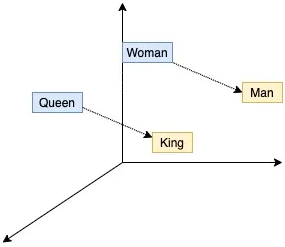
\includegraphics[width=0.3\textwidth]{word2vec.png}
    \vspace{-0.5em}
    \source{https://towardsdatascience.com/word2vec-research-paper-explained-205cb7eecc30}
\end{figure} \pause
\vspace{-0.5em}

\begin{itemize}
    \item Doc2Vec extends Word2Vec to entire documents and outperforms LDA in textbook content linkage tasks \parencites{thaker2018}
\end{itemize}

\end{frame}


\begin{frame} \frametitle{Bidirectional Encoder Representations from Transformers (BERT)}

\begin{itemize}
    \item uses two unsupervised tasks for pre-training:
    \begin{itemize} \itemsep0em
        \item masked token prediction
        \item next sentence prediction
    \end{itemize} 
    \parencites{devlin2019} \pause
    \item effectively used for automatic keyword extraction from textbooks \\ \parencites{alpizarchacon2023a}
\end{itemize}

\end{frame}


\begin{frame} \frametitle{Recurrent Neural Networks (RNNs)}

\begin{itemize}
    \item a deep neural network with capacity to remember sequences in the data. \pause
    \item can face the `vanishing gradient problem', whereby the gradient becomes too small for effective learning of long-range dependencies \\ \parencites{bengio1994} \pause
    \item Long Short-Term Memory (LSTM) networks introduced to overcome this limitation \\ \parencites{hochreiter1997}
\end{itemize}

\end{frame}


\begin{frame} \frametitle{Semantic Similarity}

\begin{itemize}
    \item refers to the degree to which two pieces of text are alike in meaning or content \pause
    \item can be measured through cosine similarity $S_C$, where documents are represented by $n$-dimensional vectors, $\textbf{a}$ and $\textbf{b}$,
    \[ S_C(\textbf{a}, \textbf{b}) := \cos(\theta) = \frac{\textbf{a} \cdot \textbf{b}}{\|\textbf{a}\| \|\textbf{b}\|} \]
\end{itemize}

\end{frame}


\begin{frame} \frametitle{Linking Multiple Textbooks}

\begin{itemize}
    \item \textbf{Topic Aggregation:} Only compute the topic vectors for the sections at lowest level in the hierarchy, and for higher levels, aggregate topic vectors by taking a weighted average of sub-topic vectors. \pause
    \item \textbf{Re-Indexing:} Compute the topic vector for every section by considering a section’s ‘document’ to be the content of the section and all it’s sub-sections.
    \item \cites{guerra2013}
\end{itemize}

\end{frame}


\section{Methodology}

\begin{frame} \frametitle{Methodology}

\begin{figure}[h]
\centering
\caption*{Architecture for topic representation and classification}
\vspace{0.1cm}
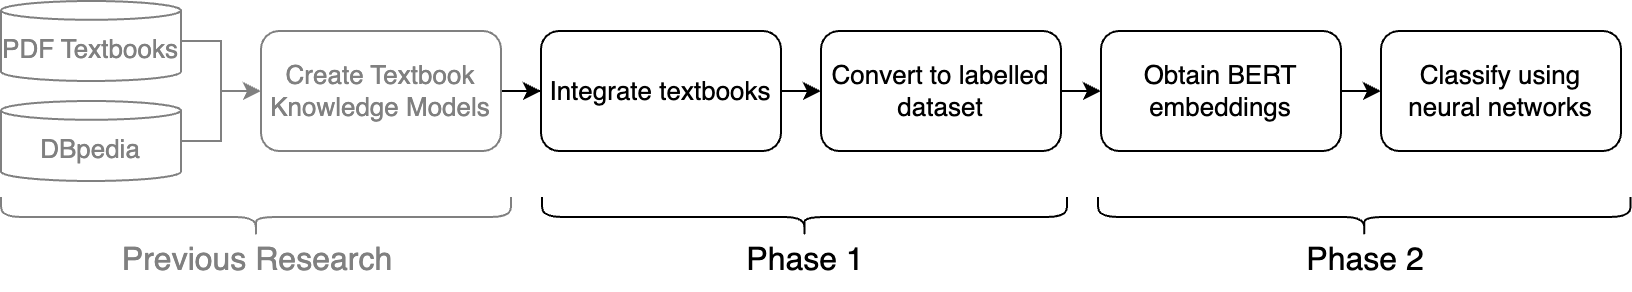
\includegraphics[width=1\textwidth]{simple-architecture.png}
\label{fig:architecture}
\end{figure}

\end{frame}


\begin{frame} \frametitle{Dataset Generation (Phase 1)}

\begin{figure}
    \centering
    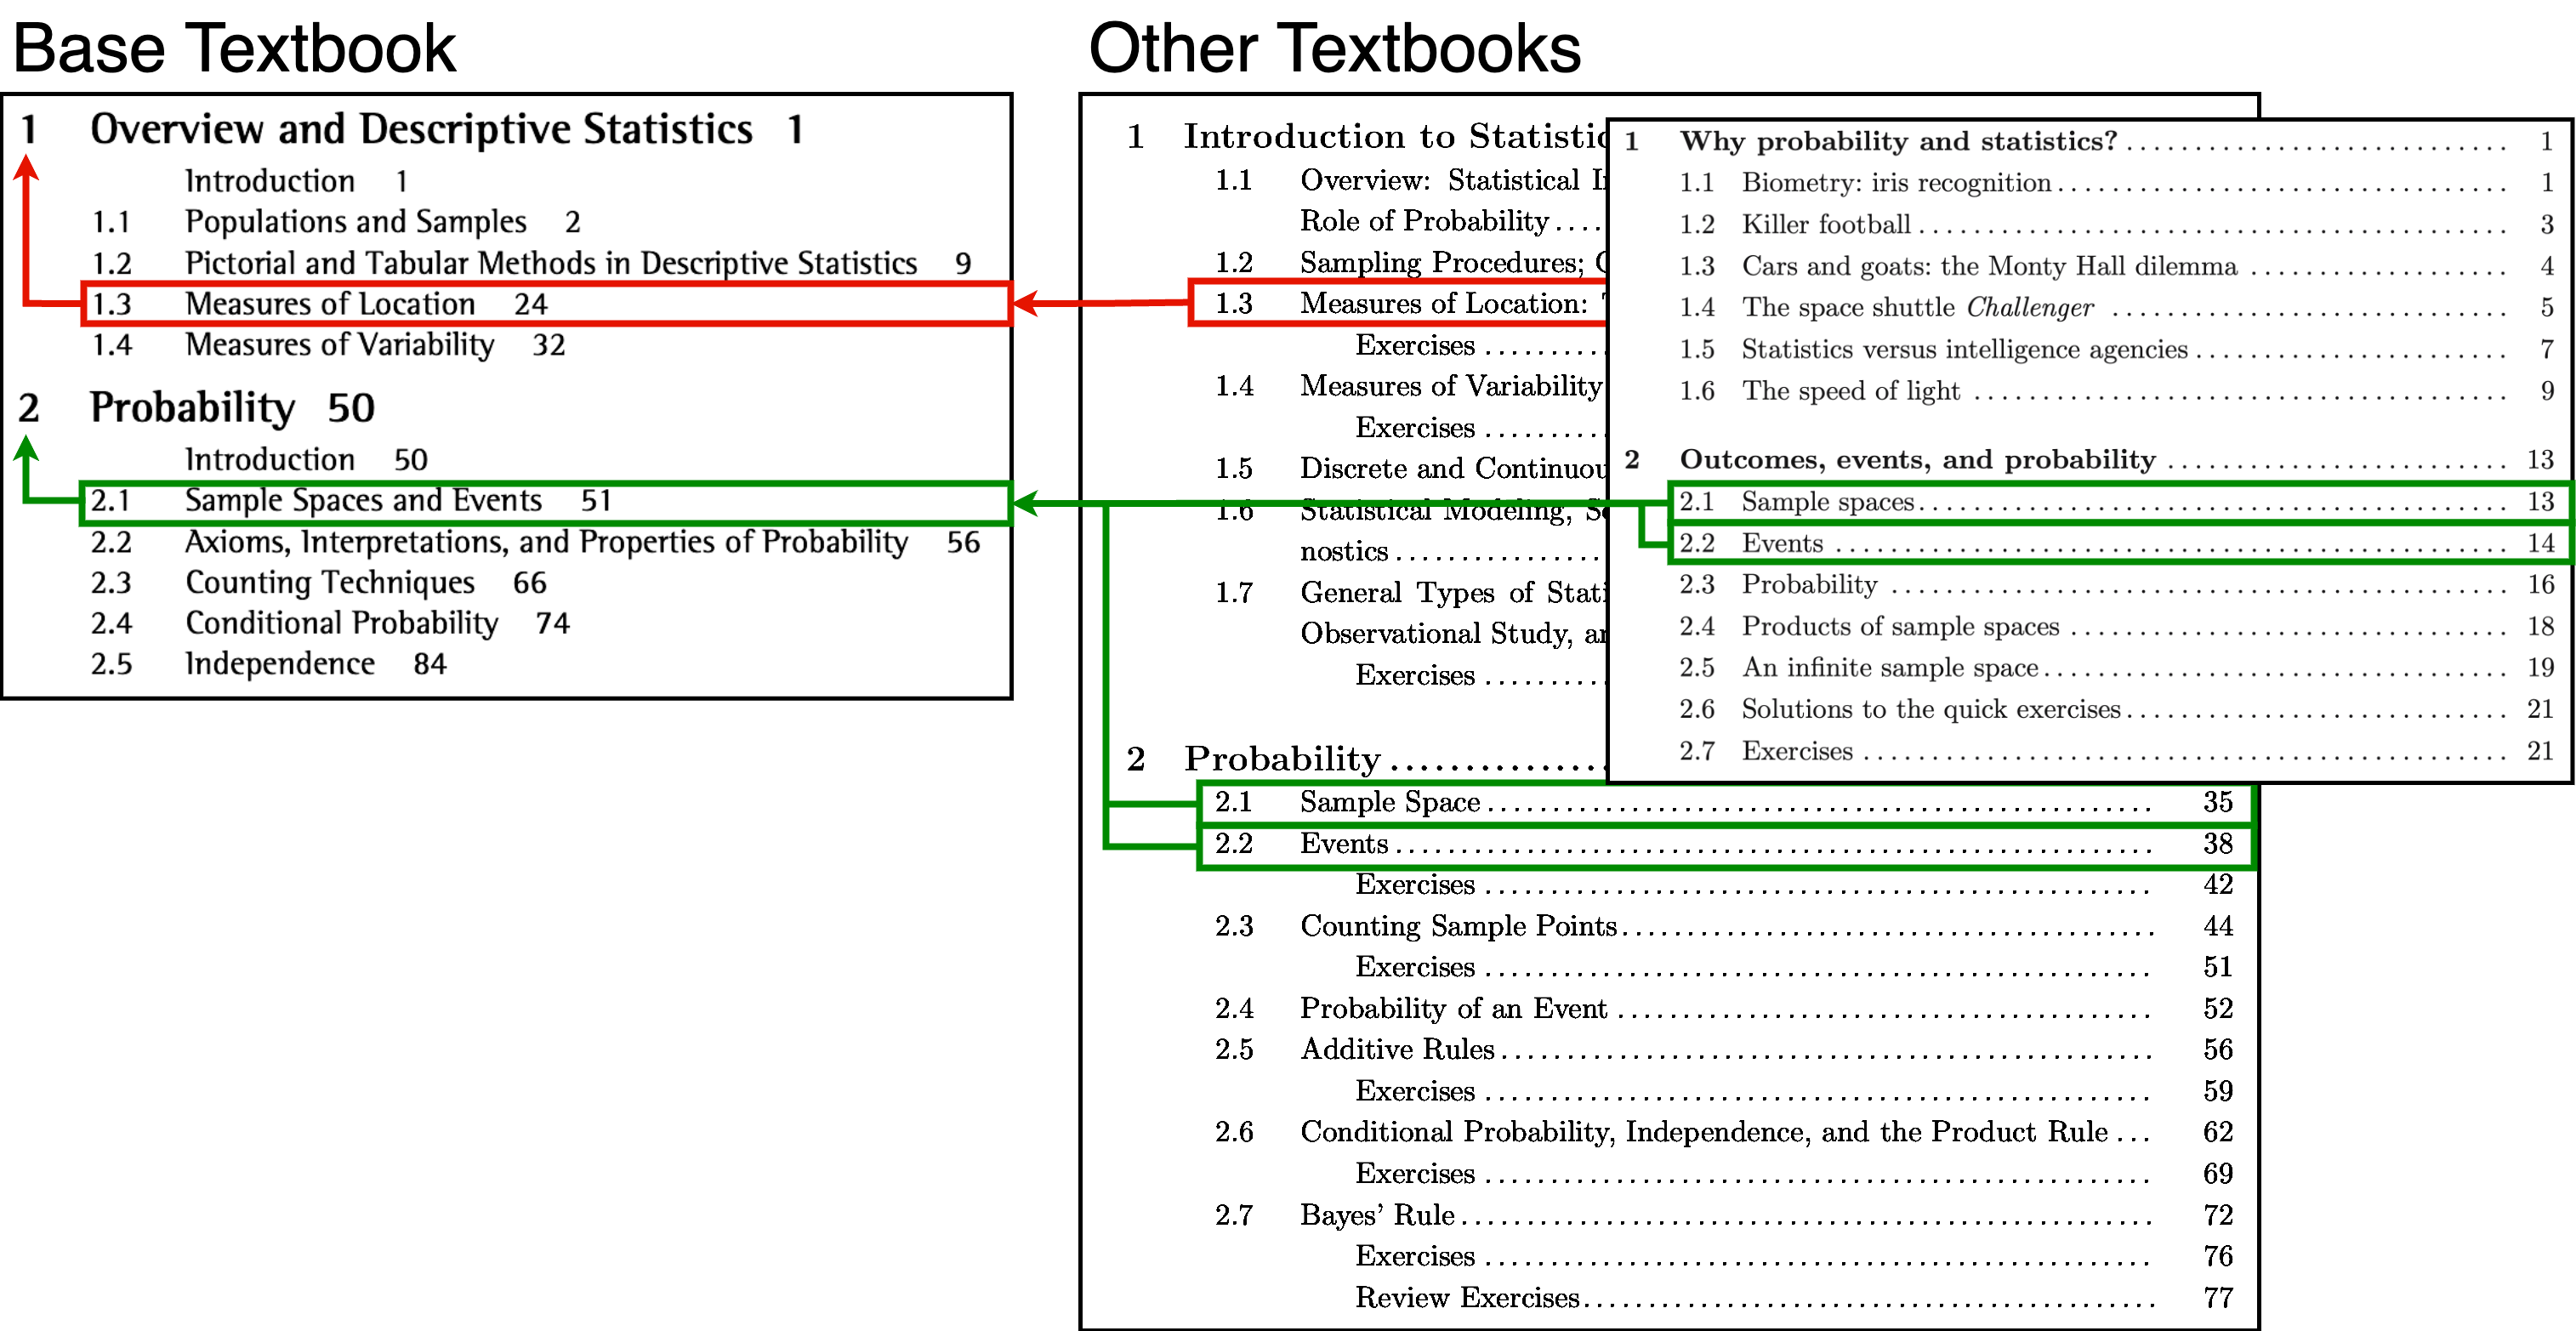
\includegraphics[width=1\textwidth]{integration.png}
\end{figure}

\end{frame}


\begin{frame} \frametitle{Dataset Generation (Phase 1)}

\begin{itemize}
    \item use multiple attributes for each section
    \begin{itemize} \itemsep0em
        \item header
        \item content
        \item concept names, definitions, concept subjects
    \end{itemize} 
    \item quick, inexpensive way to generate dataset of sections and their topics
\end{itemize}

\end{frame}

\begin{frame} \frametitle{Dataset Generation (Phase 1) – Strategies}

\begin{itemize}
    \item TF-IDF
    \item Doc2Vec
    \item Clustering
    \item Ensemble Modelling
    \begin{itemize}
        \item combination of TF-IDF and clustering
    \end{itemize}
    \item TF-IDF \& Doc2Vec Hybrid Approach
    \begin{itemize}
        \item first check for matches using TF-IDF, then use Doc2Vec for uncertain matches
    \end{itemize}
    \item Iterative Learning
    \begin{itemize}
        \item recompute section's vector after each match
    \end{itemize}
\end{itemize}

\end{frame}


\begin{frame} \frametitle{Topic Classification (Phase 2)}

\begin{itemize}
    \item goal: learn from the generated dataset to classify new content by topic \pause
    \item input text is preprocessed, tokenised, and pass to DistilBERT to generate vectors \pause
    \item RNNs are trained to classify sections into topics
\end{itemize}

\end{frame}


\section{Evaluation}


\begin{frame} \frametitle{Evaluation – Dataset Generation (Phase 1)}

\begin{itemize}
    \item evaluate performance using manual mapping generated by experts \pause
    \item false positives can have a greater cost than false negatives \\ $\implies$ precision more important than recall for this task \pause
    \item therefore, use the $F_\beta$ score with $\beta=0.5$
\end{itemize}

\end{frame}


\begin{frame} \frametitle{Evaluation – Dataset Generation (Phase 1)}


\begin{table}[h]
\centering
\caption{Summary of results for all textbook integration methods}
\label{table:phase1-results}
\begin{tabular}{lcccc}
\toprule
name & precision & recall & $F_1$ & $F_\beta$ \\
\midrule
Hybrid Model & \textbf{0.8333} & 0.3169 & 0.4592 & \textbf{0.6285} \\
Doc2Vec & 0.5714 & \textbf{0.3944} & \textbf{0.4667} & 0.5243 \\
TF-IDF & 0.5926 & 0.3380 & 0.4305 & 0.5150 \\
Ensemble & 0.4632 & 0.3099 & 0.3713 & 0.4215 \\
Clustering & 0.0260 & 0.0282 & 0.0270 & 0.0264 \\
\bottomrule
\end{tabular}
\end{table}

\begin{center}
\scriptsize
more detailed results available at GitHub repository: \\
\url{https://github.com/CobySim01/textbook-topic-analysis}
\end{center}

\end{frame}


\begin{frame} \frametitle{Evaluation – Topic Classification (Phase 2)}
\begin{itemize}
    \item expert dataset
    \begin{itemize}\itemsep0em
        \item 14 class labels
        \item 216 data points
    \end{itemize}
    \item small dataset
    \begin{itemize}\itemsep0em
        \item 32 class labels
        \item 352 data points
    \end{itemize}
    \item large generated dataset
    \begin{itemize}\itemsep0em
        \item 329 class labels
        \item 2371 data points
    \end{itemize}
\end{itemize}
\end{frame}


\begin{frame} \frametitle{Evaluation – Topic Classification (Phase 2)}

\begin{table}[h]
\centering
\caption{Summary of cross-validation performance for each dataset}
\label{table:phase2-results}
\begin{adjustbox}{center}
\resizebox{0.95\textwidth}{!}{
\begin{tabular}{lccccccccc}
\toprule
\multirow{2}{*}{dataset} & \multirow{2}{*}{concepts} & \multicolumn{2}{c}{accuracy} & \multicolumn{2}{c}{precision} & \multicolumn{2}{c}{recall} & \multicolumn{2}{c}{$F_1$} \\
 &  & model & baseline & model & baseline & model & baseline & model & baseline \\
\midrule
expert & true & \textbf{0.59} & 0.13 & \textbf{0.67} & 0.07 & \textbf{0.59} & 0.13 & 0.61 & 0.08 \\
expert & false & 0.41 & 0.13 & 0.50 & 0.09 & 0.41 & 0.13 & 0.44 & 0.09 \\
small & true & 0.35 & 0.05 & 0.48 & 0.03 & 0.35 & 0.05 & 0.53 & 0.04 \\
small & false & 0.45 & 0.05 & 0.64 & 0.03 & 0.45 & 0.05 & \textbf{0.62} & 0.04 \\
large & true & 0.26 & 0.00 & 0.56 & 0.00 & 0.26 & 0.00 & 0.40 & 0.00 \\
large & false & 0.24 & 0.00 & 0.57 & 0.00 & 0.24 & 0.00 & 0.37 & 0.00 \\
\bottomrule
\end{tabular}
}
\end{adjustbox}
\end{table}

\end{frame}


\section{Discussion}

\begin{frame} \frametitle{Limitations}

\begin{itemize}
    \item quality issues with generated dataset limit the performance of topic classification \pause
    \item pre-trained model from Hugging Face is not fully tailored to our needs \pause
    \item classes are too broad, since top-level sections are used
\end{itemize}

\end{frame}


\begin{frame} \frametitle{Key Takeaways}

\begin{itemize}
    \item a wide variety of research into this area already exists \pause
    \item we propose a novel architecture to develop a domain-dependent and fine-grained topic model \pause
    \item initial results justify further research and investments to improve the architecture
\end{itemize}

\end{frame}





%------------------------------------------------

\begin{frame}[allowframebreaks]
\frametitle{References}
    \printbibliography
\end{frame}

\begin{frame} \frametitle{Appendix}

\begin{table}[h]
\centering
\caption{Selected parameters for each dataset}
\label{table:phase-2-results-a}
\begin{tabular}{lllrrr}
\toprule
dataset & concepts & model type & batch size & dropout rate & units \\
\midrule
expert & true & SimpleRNN & 128 & 0.40 & 125 \\
expert & false & LSTM & 128 & 0.40 & 200 \\
small & true & SimpleRNN & 32 & 0.90 & 100 \\
small & false & SimpleRNN & 64 & 0.90 & 100 \\
large & true & SimpleRNN & 64 & 0.90 & 125 \\
large & false & SimpleRNN & 64 & 0.90 & 100 \\
\bottomrule
\end{tabular}
\end{table}



\end{frame}

%----------------------------------------------------------------------------------------

\end{document} 
